For the third iteration was the goal to remove the raycasting that happens on runtime and to add other potential performance improvements.

\subsection*{Minimizing the Graph size}
It was possible to reduce the number of waypoints even further.
In order to do so all waypoints are looped through to find adjacent waypoints, meaning waypoints whose distance to each other is less or equal to one.
Those that are adjacent are then removed and a new waypoint is placed halfway between them.
This is illustrated in Figure \ref{waypointMerge}.
The resulting waypoints can be seen in Figure \ref{waypointOpt} with the graph in Figure \ref{waypointgraphOpt}. 
This can be compared to the old waypoint figure and graph shown in Figure \ref{waypointsNode} and Figure \ref{waypointgraph}.
Most notably, the amount of edges are significantly reduced.
\begin{figure}[H]
\begin{center}
	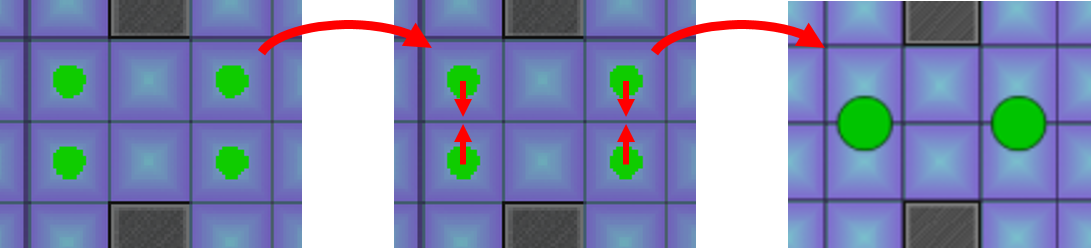
\includegraphics[width=\textwidth]{figures/astar/waypointMerge}
	\caption{Waypoint merging.}
	\label{waypointMerge}
\end{center}
\end{figure}

\begin{figure}[H]
\centering
	\begin{minipage}{.5\textwidth}
		\centering
		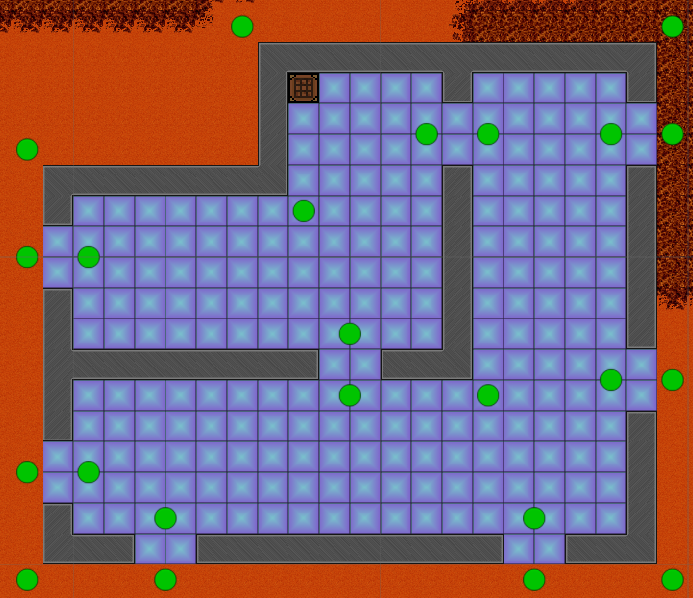
\includegraphics[scale=0.3]{figures/astar/optimizedWaypoints}
		\captionof{figure}{Waypoints after merge optimizations.}
		\label{waypointOpt}
	\end{minipage}%
	\begin{minipage}{.5\textwidth}
		\centering
		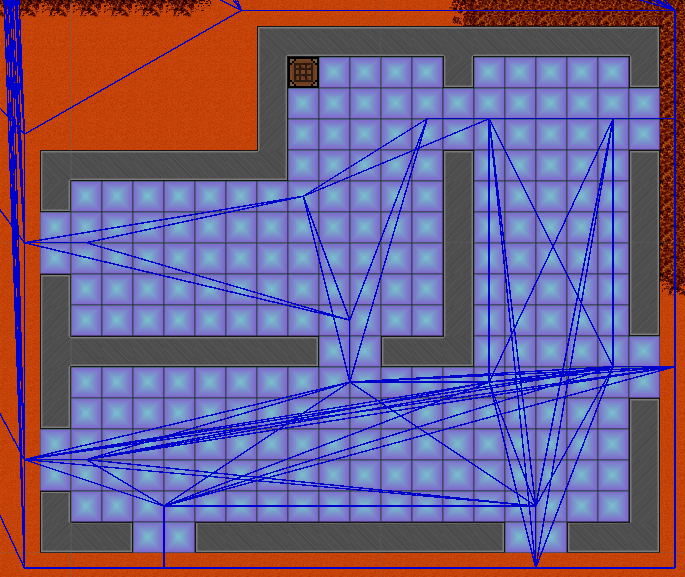
\includegraphics[scale=0.315]{figures/astar/optimizedWaypointsGraph}
		\captionof{figure}{Graph based on the waypoints after waypoint optimization.}
		\label{waypointgraphOpt}
	\end{minipage}
\end{figure}

\subsection*{Eliminating raycasts}
Raycast, in this case, is used to test if there is a straight, unobstructed path between two points in the game world.
This happens in two places:
\begin{itemize}
\item Between the positions of enemies and players
\item Between the positions of enemies and waypoints
\end{itemize}
The raycast from an enemy to a player happens when the enemy want to check if the enemy can ``see'' the player, i.e. the path to the player is unobstructed.
To prevent the raycast checks to the players, the map is partitioned into convex rectangles.
When an enemy then enters the same partition as a player it knows that it can walk directly towards the player since the rectangle is convex.
Such partitions are generated while also generating the backdrop.
For finding the rectangles to use for partitions, an inverted version of the algorithm used to walls, is used to find areas that are non-walls.
The resulting partitions of running the algorithm is illustrated in Figure~\ref{fig:partition_colliders_on_map}.

\begin{figure}[H]
\begin{center}
        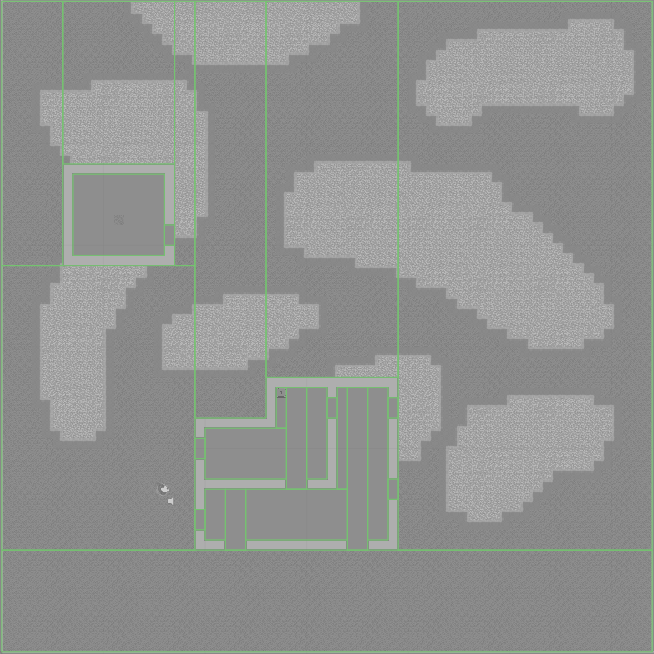
\includegraphics[width=0.9\textwidth]{figures/generating_levels/partition_colliders.png}
    \caption{Rectangles for partitions, separated by green lines.}\label{fig:partition_colliders_on_map}
\end{center}
\end{figure}

Once the partitions are made, trigger colliders are added to them.
Once a player or enemy collides with a partition, they will add a reference to that partition to their list of partitions.
Once they stop colliding with the partition they will remove it from their list of partitions.

\subsubsection*{Use of Partitions}
The enemy starts by checking whether it and the player are in the same partition and if so the enemy can go straight towards the player and the enemy will be in hunting mode.
In hunting mode, the enemy can also check neighbouring partitions for the player, such that if the player runs out of the partition, the enemy will still go straight towards the player.
This prevents odd behaviour from the enemies when they chase a players, since if there was no hunting mode the enemy would have to start pathfinding if the player leaves the partition, as illustrated in Figure \ref{huntingMode}.

\begin{figure}[H]
\begin{center}
        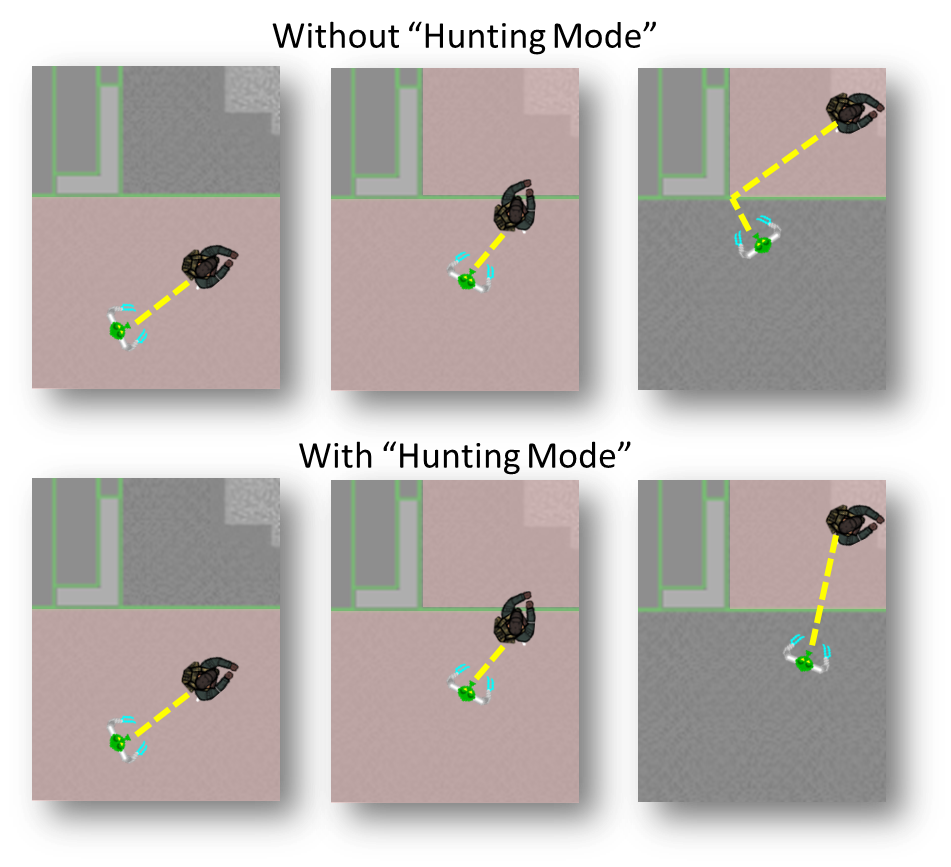
\includegraphics[width=\textwidth]{figures/astar/huntingMode.png}
    \caption{Behaviour difference between hunting mode and no hunting mode, showing if the players leave a partition the enemy without hunting mode would have to start pathfinding resulting in odd behaviour.}\label{huntingMode}
\end{center}
\end{figure}

If the player then escapes, meaning that the player is not in the same nor a neighbouring partitions, the enemy will start to run the pathfinding algorithm and follow the path.
The enemy will then run pathfinding again in $X$ seconds, where $X = \text{number of nodes in the path}$.
This is to recalculate the path in case the player has moved elsewhere since last run.
It is based on the number of nodes because that means enemies that aren't close to the player (and thus out of sight) will not take up as many resources.
The pathfinding continues until the enemy is in the same partition as the player again.

Running A* continuously while having a 50 enemies or more was still costly.
Therefore, the A* was moved to load time where it finds the shortest path for all the possible paths, and saves it in a hashtable.
That way, the pathfinding used during runtime is only lookups in the hashtable.
This is possible due to our relative low number of nodes and edges.\\
The last optimization was to eliminate the costly raycast happening when finding the nearest waypoints. 
This is done by adding the waypoints from the partition of the enemy and its neighbouring partitions into a list, then finding the one with the shortest distance. 
This ensures the closest accessible waypoint is found.

\subsection*{Result}
The result of this iteration was that all raycasting was removed from runtime and some of these raycasts were moved to load-time instead.
Furthermore A* calculations were moved to load-time which together with the waypoint-merge-optimization made the pathfinding algorithm work very effective, allowing us to reach a greater number of active enemies.

The trade-off from this improved performance is present if the player can move too quickly through partitions with a low number of waypoints.
As illustrated in Figure \ref{tradeoff}, the enemy can only hunt through two partitions, which leads to the enemy having odd looking behaviour if the player runs too quickly through the partitions.
\begin{figure}[H]
\begin{center}
        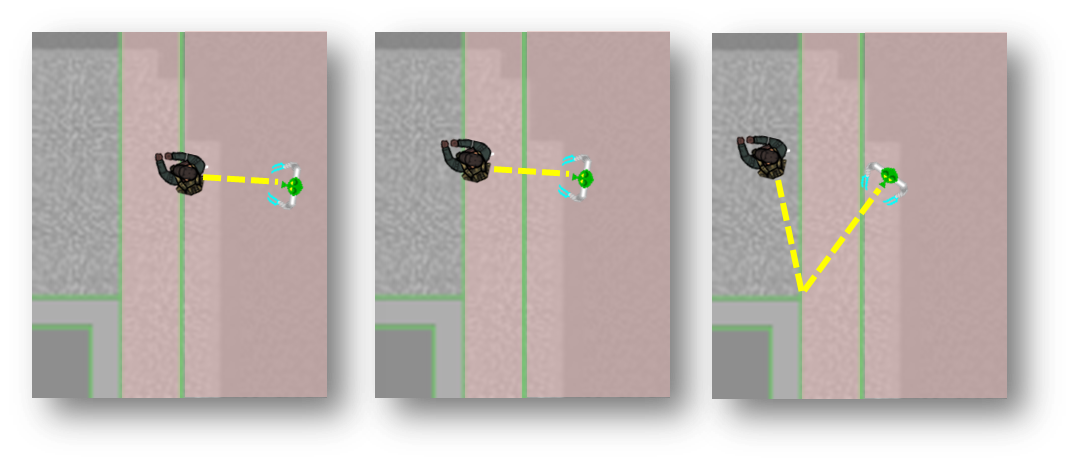
\includegraphics[width=\textwidth]{figures/astar/tradeoff.png}
    \caption{Illustration of the problem with small partitions with low waypoint count. Red partitions shows the partitions of the enemy.}\label{tradeoff}
\end{center}
\end{figure}